% Options for packages loaded elsewhere
% Options for packages loaded elsewhere
\PassOptionsToPackage{unicode}{hyperref}
\PassOptionsToPackage{hyphens}{url}
%
\documentclass[
  ignorenonframetext,
  aspectratio=169,
  11pt]{beamer}
\newif\ifbibliography
\usepackage{pgfpages}
\setbeamertemplate{caption}[numbered]
\setbeamertemplate{caption label separator}{: }
\setbeamercolor{caption name}{fg=normal text.fg}
\beamertemplatenavigationsymbolsempty
% remove section numbering
\setbeamertemplate{part page}{
  \centering
  \begin{beamercolorbox}[sep=16pt,center]{part title}
    \usebeamerfont{part title}\insertpart\par
  \end{beamercolorbox}
}
\setbeamertemplate{section page}{
  \centering
  \begin{beamercolorbox}[sep=12pt,center]{section title}
    \usebeamerfont{section title}\insertsection\par
  \end{beamercolorbox}
}
\setbeamertemplate{subsection page}{
  \centering
  \begin{beamercolorbox}[sep=8pt,center]{subsection title}
    \usebeamerfont{subsection title}\insertsubsection\par
  \end{beamercolorbox}
}
% Prevent slide breaks in the middle of a paragraph
\widowpenalties 1 10000
\raggedbottom
\AtBeginPart{
  \frame{\partpage}
}
\AtBeginSection{
  \ifbibliography
  \else
    \frame{\sectionpage}
  \fi
}
\AtBeginSubsection{
  \frame{\subsectionpage}
}
\usepackage{iftex}
\ifPDFTeX
  \usepackage[T1]{fontenc}
  \usepackage[utf8]{inputenc}
  \usepackage{textcomp} % provide euro and other symbols
\else % if luatex or xetex
  \usepackage{unicode-math} % this also loads fontspec
  \defaultfontfeatures{Scale=MatchLowercase}
  \defaultfontfeatures[\rmfamily]{Ligatures=TeX,Scale=1}
\fi
\usepackage{lmodern}

\usetheme[]{metropolis}
\usecolortheme[]{default}
\usefonttheme[]{default}
\ifPDFTeX\else
  % xetex/luatex font selection
\fi
% Use upquote if available, for straight quotes in verbatim environments
\IfFileExists{upquote.sty}{\usepackage{upquote}}{}
\IfFileExists{microtype.sty}{% use microtype if available
  \usepackage[]{microtype}
  \UseMicrotypeSet[protrusion]{basicmath} % disable protrusion for tt fonts
}{}
\makeatletter
\@ifundefined{KOMAClassName}{% if non-KOMA class
  \IfFileExists{parskip.sty}{%
    \usepackage{parskip}
  }{% else
    \setlength{\parindent}{0pt}
    \setlength{\parskip}{6pt plus 2pt minus 1pt}}
}{% if KOMA class
  \KOMAoptions{parskip=half}}
\makeatother

\usepackage{color}
\usepackage{fancyvrb}
\newcommand{\VerbBar}{|}
\newcommand{\VERB}{\Verb[commandchars=\\\{\}]}
\DefineVerbatimEnvironment{Highlighting}{Verbatim}{commandchars=\\\{\}}
% Add ',fontsize=\small' for more characters per line
\usepackage{framed}
\definecolor{shadecolor}{RGB}{241,243,245}
\newenvironment{Shaded}{\begin{snugshade}}{\end{snugshade}}
\newcommand{\AlertTok}[1]{\textcolor[rgb]{0.68,0.00,0.00}{#1}}
\newcommand{\AnnotationTok}[1]{\textcolor[rgb]{0.37,0.37,0.37}{#1}}
\newcommand{\AttributeTok}[1]{\textcolor[rgb]{0.40,0.45,0.13}{#1}}
\newcommand{\BaseNTok}[1]{\textcolor[rgb]{0.68,0.00,0.00}{#1}}
\newcommand{\BuiltInTok}[1]{\textcolor[rgb]{0.00,0.23,0.31}{#1}}
\newcommand{\CharTok}[1]{\textcolor[rgb]{0.13,0.47,0.30}{#1}}
\newcommand{\CommentTok}[1]{\textcolor[rgb]{0.37,0.37,0.37}{#1}}
\newcommand{\CommentVarTok}[1]{\textcolor[rgb]{0.37,0.37,0.37}{\textit{#1}}}
\newcommand{\ConstantTok}[1]{\textcolor[rgb]{0.56,0.35,0.01}{#1}}
\newcommand{\ControlFlowTok}[1]{\textcolor[rgb]{0.00,0.23,0.31}{\textbf{#1}}}
\newcommand{\DataTypeTok}[1]{\textcolor[rgb]{0.68,0.00,0.00}{#1}}
\newcommand{\DecValTok}[1]{\textcolor[rgb]{0.68,0.00,0.00}{#1}}
\newcommand{\DocumentationTok}[1]{\textcolor[rgb]{0.37,0.37,0.37}{\textit{#1}}}
\newcommand{\ErrorTok}[1]{\textcolor[rgb]{0.68,0.00,0.00}{#1}}
\newcommand{\ExtensionTok}[1]{\textcolor[rgb]{0.00,0.23,0.31}{#1}}
\newcommand{\FloatTok}[1]{\textcolor[rgb]{0.68,0.00,0.00}{#1}}
\newcommand{\FunctionTok}[1]{\textcolor[rgb]{0.28,0.35,0.67}{#1}}
\newcommand{\ImportTok}[1]{\textcolor[rgb]{0.00,0.46,0.62}{#1}}
\newcommand{\InformationTok}[1]{\textcolor[rgb]{0.37,0.37,0.37}{#1}}
\newcommand{\KeywordTok}[1]{\textcolor[rgb]{0.00,0.23,0.31}{\textbf{#1}}}
\newcommand{\NormalTok}[1]{\textcolor[rgb]{0.00,0.23,0.31}{#1}}
\newcommand{\OperatorTok}[1]{\textcolor[rgb]{0.37,0.37,0.37}{#1}}
\newcommand{\OtherTok}[1]{\textcolor[rgb]{0.00,0.23,0.31}{#1}}
\newcommand{\PreprocessorTok}[1]{\textcolor[rgb]{0.68,0.00,0.00}{#1}}
\newcommand{\RegionMarkerTok}[1]{\textcolor[rgb]{0.00,0.23,0.31}{#1}}
\newcommand{\SpecialCharTok}[1]{\textcolor[rgb]{0.37,0.37,0.37}{#1}}
\newcommand{\SpecialStringTok}[1]{\textcolor[rgb]{0.13,0.47,0.30}{#1}}
\newcommand{\StringTok}[1]{\textcolor[rgb]{0.13,0.47,0.30}{#1}}
\newcommand{\VariableTok}[1]{\textcolor[rgb]{0.07,0.07,0.07}{#1}}
\newcommand{\VerbatimStringTok}[1]{\textcolor[rgb]{0.13,0.47,0.30}{#1}}
\newcommand{\WarningTok}[1]{\textcolor[rgb]{0.37,0.37,0.37}{\textit{#1}}}

\usepackage{longtable,booktabs,array}
\newcounter{none} % for unnumbered tables
\usepackage{calc} % for calculating minipage widths
\usepackage{caption}
% Make caption package work with longtable
\makeatletter
\def\fnum@table{\tablename~\thetable}
\makeatother
\usepackage{graphicx}
\makeatletter
\newsavebox\pandoc@box
\newcommand*\pandocbounded[1]{% scales image to fit in text height/width
  \sbox\pandoc@box{#1}%
  \Gscale@div\@tempa{\textheight}{\dimexpr\ht\pandoc@box+\dp\pandoc@box\relax}%
  \Gscale@div\@tempb{\linewidth}{\wd\pandoc@box}%
  \ifdim\@tempb\p@<\@tempa\p@\let\@tempa\@tempb\fi% select the smaller of both
  \ifdim\@tempa\p@<\p@\scalebox{\@tempa}{\usebox\pandoc@box}%
  \else\usebox{\pandoc@box}%
  \fi%
}
% Set default figure placement to htbp
\def\fps@figure{htbp}
\makeatother


% definitions for citeproc citations
\NewDocumentCommand\citeproctext{}{}
\NewDocumentCommand\citeproc{mm}{%
  \begingroup\def\citeproctext{#2}\cite{#1}\endgroup}
\makeatletter
 % allow citations to break across lines
 \let\@cite@ofmt\@firstofone
 % avoid brackets around text for \cite:
 \def\@biblabel#1{}
 \def\@cite#1#2{{#1\if@tempswa , #2\fi}}
\makeatother
\newlength{\cslhangindent}
\setlength{\cslhangindent}{1.5em}
\newlength{\csllabelwidth}
\setlength{\csllabelwidth}{3em}
\newenvironment{CSLReferences}[2] % #1 hanging-indent, #2 entry-spacing
 {\begin{list}{}{%
  \setlength{\itemindent}{0pt}
  \setlength{\leftmargin}{0pt}
  \setlength{\parsep}{0pt}
  % turn on hanging indent if param 1 is 1
  \ifodd #1
   \setlength{\leftmargin}{\cslhangindent}
   \setlength{\itemindent}{-1\cslhangindent}
  \fi
  % set entry spacing
  \setlength{\itemsep}{#2\baselineskip}}}
 {\end{list}}
\usepackage{calc}
\newcommand{\CSLBlock}[1]{\hfill\break\parbox[t]{\linewidth}{\strut\ignorespaces#1\strut}}
\newcommand{\CSLLeftMargin}[1]{\parbox[t]{\csllabelwidth}{\strut#1\strut}}
\newcommand{\CSLRightInline}[1]{\parbox[t]{\linewidth - \csllabelwidth}{\strut#1\strut}}
\newcommand{\CSLIndent}[1]{\hspace{\cslhangindent}#1}



\setlength{\emergencystretch}{3em} % prevent overfull lines

\providecommand{\tightlist}{%
  \setlength{\itemsep}{0pt}\setlength{\parskip}{0pt}}



 


% ---------- Packages ----------
\usepackage{booktabs}
\usepackage{etoolbox}

% ---------- Emory palette ----------
\definecolor{emoryblue}{HTML}{1E376D}
\definecolor{emorygold}{HTML}{D9AB28}
\definecolor{emorygolddark}{HTML}{8A5A00}
\definecolor{textcharcoal}{HTML}{20242B}
\definecolor{secondarygray}{HTML}{667085}
\definecolor{lightpanel}{HTML}{F2F5F8}
\definecolor{rulegray}{HTML}{D9DEE5}
\definecolor{softgold}{HTML}{FBF5E6}

% ---------- Global appearance ----------
\setbeamercolor{normal text}{fg=textcharcoal,bg=white}
\setbeamercolor{structure}{fg=emoryblue}
\setbeamercolor{alerted text}{fg=emorygolddark}
\setbeamercolor{background canvas}{bg=white}
\setbeamercolor{page number in head/foot}{
  fg=secondarygray,
  bg=white
}

\setbeamerfont{title}{
  series=\bfseries,
  size=\LARGE
}

\setbeamerfont{subtitle}{
  shape=\itshape,
  size=\large
}

\setbeamerfont{frametitle}{
  series=\bfseries,
  size=\Large
}

\setbeamerfont{section title}{
  series=\bfseries,
  size=\huge
}

\setbeamerfont{block title}{
  series=\bfseries
}

\setbeamerfont{page number in head/foot}{
  size=\scriptsize
}

\setbeamersize{
  text margin left=0.60cm,
  text margin right=0.60cm
}

\setbeamertemplate{navigation symbols}{}

\setbeamercolor{title}{
  fg=emoryblue,
  bg=white
}

\setbeamercolor{subtitle}{
  fg=textcharcoal,
  bg=white
}

\setbeamercolor{author}{
  fg=textcharcoal,
  bg=white
}

\setbeamercolor{institute}{
  fg=secondarygray,
  bg=white
}

\setbeamercolor{date}{
  fg=secondarygray,
  bg=white
}

\setbeamercolor{title separator}{
  fg=emorygold
}

\setbeamertemplate{title separator}{%
  \par
  \kern0.55em
  {\color{emorygold}\rule{2.2cm}{1.2pt}}
  \par
  \kern0.55em
}

% Reserve a dedicated column for the logo so that long titles cannot
% overlap it.
\makeatletter
\setbeamertemplate{title page}{%
  % Filling the frame height prevents Beamer's default vertical centering
  % from pushing this composition back toward the middle of the slide.
  \vbox to 0.88\textheight{%
    \vspace*{0.45cm}
    \begin{columns}[T,onlytextwidth]
      \begin{column}{0.72\textwidth}
        \vbox to 0.80\textheight{%
          \vspace*{0.55cm}
          \ifx\inserttitle\@empty\else
            {\usebeamerfont{title}\usebeamercolor[fg]{title}\inserttitle\par}
            \usebeamertemplate*{title separator}
          \fi
          \ifx\insertsubtitle\@empty\else
            {\usebeamerfont{subtitle}\usebeamercolor[fg]{subtitle}%
             \linespread{1.05}\selectfont\insertsubtitle\par}
          \fi
          \vfill
          \ifx\insertauthor\@empty\else
            {\usebeamerfont{author}\usebeamercolor[fg]{author}\insertauthor\par}
          \fi
          \ifx\insertdate\@empty\else
            \vspace{0pt}
            {\usebeamerfont{date}\usebeamercolor[fg]{date}\insertdate\par}
          \fi
          \ifx\insertinstitute\@empty\else
            \vspace{0.27cm}
            {\usebeamerfont{institute}\usebeamercolor[fg]{institute}\insertinstitute\par}
          \fi
          % Balance the flexible gap above the presenter details against
          % a modest lower margin; this keeps neither area oversized.
          \vspace{0.30cm}
        }
      \end{column}
      \begin{column}{0.24\textwidth}
        \vspace*{0.55cm}
        \raggedleft
        \IfFileExists{ShieldEmory_hz_280_pres2023.png}{%
          
\includegraphics[width=\linewidth]{ShieldEmory_hz_280_pres2023.png}%
        }{}
      \end{column}
    \end{columns}
    \vfill
  }
}
\makeatother

% ---------- Compact full-width frame title bar ----------
\setbeamercolor{frametitle}{
  fg=white,
  bg=emoryblue
}

\setbeamertemplate{frametitle}{%
  \nointerlineskip
  \begin{beamercolorbox}[
    wd=\paperwidth,
    sep=0.20cm,
    leftskip=0.15cm,
    rightskip=0.15cm
  ]{frametitle}
    \usebeamerfont{frametitle}
    \strut\insertframetitle\strut
  \end{beamercolorbox}
}

% ---------- Section dividers ----------
\setbeamercolor{section page}{
  fg=white,
  bg=emoryblue
}

\setbeamertemplate{section page}{%
  \centering
  {\usebeamerfont{section title}\usebeamercolor[fg]{section page}%
   \insertsection\par}
  \vspace{0.22cm}
  {\color{emorygold}\rule{2.2cm}{0.8pt}\par}
}

\AtBeginSection[]{%
  \begingroup
    \setbeamercolor{background canvas}{bg=emoryblue}
    \begin{frame}[
      plain,
      noframenumbering,
      c
    ]
      \sectionpage
    \end{frame}
  \endgroup
}

% ---------- Lists ----------
\setbeamertemplate{itemize item}{%
  \color{emorygold}
  \raisebox{0.12em}{
    \scriptsize$\bullet$
  }
}

\setbeamertemplate{itemize subitem}{%
  \color{emoryblue}
  \raisebox{0.08em}{
    \tiny$\bullet$
  }
}

\setbeamertemplate{enumerate item}{%
  \color{emoryblue}
  \insertenumlabel.
}

% ---------- Blocks ----------
% Use Beamer's native rounded shadow so the complete lower and right
% perimeter is covered. Reduce opacity at the shadow-fill stage; changing
% beamer@safeblack would also recolor Beamer's clipping mask.
\makeatletter
\patchcmd{\endbeamerboxesrounded}
  {\pgfsetfillcolor{beamer@safeblack}}
  {\pgfsetfillcolor{beamer@safeblack}%
   \pgfsetfillopacity{0.24}}
  {}
  {\PackageWarning{emory-theme}{Could not reduce block shadow opacity}}
\makeatother
\setbeamertemplate{blocks}[rounded][shadow=true]

% Standard block: blue heading, pale blue body
\setbeamercolor{block title}{
  fg=white,
  bg=emoryblue
}

\setbeamercolor{block body}{
  fg=textcharcoal,
  bg=lightpanel
}

% Alert block: gold heading, pale gold body
\setbeamercolor{block title alerted}{
  fg=textcharcoal,
  bg=emorygold
}

\setbeamercolor{block body alerted}{
  fg=textcharcoal,
  bg=softgold
}

% Example block: gray heading
\setbeamercolor{block title example}{
  fg=white,
  bg=secondarygray
}

\setbeamercolor{block body example}{
  fg=textcharcoal,
  bg=lightpanel
}

% ---------- Footer ----------
% Hides numbering on the title and section-divider slides. The main-deck
% denominator stops at the recorded boundary; appendix frames use A1/A2.
\makeatletter
\newcommand{\csdrrecordappendixboundary}{\beamer@appendixwrite}
\setbeamertemplate{footline}{%
  \leavevmode%
  \ifnum\value{framenumber}>1
    \hbox{%
      \begin{beamercolorbox}[
        wd=\paperwidth,
        ht=0.28cm,
        dp=0.16cm,
        rightskip=0.55cm
      ]{page number in head/foot}
        \hfill
        \ifnum\value{framenumber}>\insertmainframenumber\relax
          A\the\numexpr\value{framenumber}-\insertmainframenumber\relax
          \,/\,%
          A\the\numexpr\inserttotalframenumber-\insertmainframenumber\relax
        \else
          \the\numexpr\value{framenumber}-1\relax
          \,/\,%
          \the\numexpr\insertmainframenumber-1\relax
        \fi
      \end{beamercolorbox}
    }
  \fi
}
\makeatother

% ---------- Tables and code ----------
\AtBeginEnvironment{tabular}{
  \color{textcharcoal}
}

\AtBeginDocument{
  \definecolor{shadecolor}{HTML}{F2F5F8}
}

% Number standard figure captions and keep them visually secondary.
\setbeamertemplate{caption}[numbered]
\setbeamerfont{caption}{size=\small}
\setbeamercolor{caption name}{fg=secondarygray}
\setbeamercolor{caption}{fg=secondarygray}
\DeclareCaptionFont{pfasapplication}{%
  \sffamily\fontsize{7.0}{8.4}\selectfont
}

% Compact target icon for the plain-language estimand callout.
\newcommand{\targeticon}{%
  \tikz[baseline=-0.50ex,scale=0.12]{%
    \draw[emoryblue,line width=0.55pt] (0,0) circle (1);
    \draw[emoryblue,line width=0.55pt] (0,0) circle (0.58);
    \fill[emoryblue] (0,0) circle (0.17);
  }%
}

% Shared type size for all workflow-slide code and console panels.
\newcommand{\workflowcodefont}{\fontsize{6.3}{7.1}\selectfont}

% ---------- Semantic emphasis commands ----------
% Proposed method or other primary concept
\newcommand{\method}[1]{%
  \textcolor{emoryblue}{\textbf{#1}}%
}

% Focal element; safe inside equations
\newcommand{\focus}[1]{%
  \textcolor{emorygolddark}{#1}%
}

% Secondary explanation
\newcommand{\muted}[1]{%
  \textcolor{secondarygray}{#1}%
}
\makeatletter
\@ifpackageloaded{caption}{}{\usepackage{caption}}
\AtBeginDocument{%
\ifdefined\contentsname
  \renewcommand*\contentsname{Table of contents}
\else
  \newcommand\contentsname{Table of contents}
\fi
\ifdefined\listfigurename
  \renewcommand*\listfigurename{List of Figures}
\else
  \newcommand\listfigurename{List of Figures}
\fi
\ifdefined\listtablename
  \renewcommand*\listtablename{List of Tables}
\else
  \newcommand\listtablename{List of Tables}
\fi
\ifdefined\figurename
  \renewcommand*\figurename{Figure}
\else
  \newcommand\figurename{Figure}
\fi
\ifdefined\tablename
  \renewcommand*\tablename{Table}
\else
  \newcommand\tablename{Table}
\fi
}
\@ifpackageloaded{float}{}{\usepackage{float}}
\floatstyle{ruled}
\@ifundefined{c@chapter}{\newfloat{codelisting}{h}{lop}}{\newfloat{codelisting}{h}{lop}[chapter]}
\floatname{codelisting}{Listing}
\newcommand*\listoflistings{\listof{codelisting}{List of Listings}}
\makeatother
\makeatletter
\makeatother
\makeatletter
\@ifpackageloaded{caption}{}{\usepackage{caption}}
\@ifpackageloaded{subcaption}{}{\usepackage{subcaption}}
\makeatother

\usepackage{bookmark}
\IfFileExists{xurl.sty}{\usepackage{xurl}}{} % add URL line breaks if available
\urlstyle{same}
% fallback for those not using the hyperref driver hyperxmp:
\makeatletter
\@ifundefined{xmpquote}{\newcommand{\xmpquote}[1]{#1}}{}
\makeatother
\hypersetup{
  pdftitle={Causal dimension reduction for environmental health},
  pdfauthor={Thomas Hsiao, Ph.D.~},
  hidelinks,
  pdfcreator={LaTeX via pandoc}}


\title{\texorpdfstring{Causal dimension reduction for environmental
health}{Causal dimension reduction for environmental health}}
\subtitle{\texorpdfstring{Wake Forest University BDS Faculty Candidate
Talk}{Wake Forest University BDS Faculty Candidate Talk}}
\author{Thomas Hsiao,
Ph.D.~\newline \textcolor{secondarygray}{Postdoctoral Fellow}}
\date{November 4, 2026}
\institute{Emory University \newline Rollins School of Public Health
\newline Department of Biostatistics and Bioinformatics}

\begin{document}
\frame{\titlepage}


\begin{frame}{Environmental mixtures analysis}
\protect\phantomsection\label{environmental-mixtures-analysis}
\begin{columns}[c,onlytextwidth]
\begin{column}{0.55\linewidth}
How can we quantify the causal effect of complex environmental
exposures? \vspace{0.34cm}

\begin{itemize}
\tightlist
\item
  Air pollution mixtures (PM\textsubscript{2.5}, NO\textsubscript{2},
  O\textsubscript{3}, \(\ldots\))
\item
  PFAS compounds (PFOA, PFOS, PFNA, \(\ldots\))
\item
  Metals (Pb, Cd, As, Hg, \(\ldots\)) \vspace{0.34cm}
\end{itemize}

All involve multiple, highly correlated, continuous exposures
\end{column}

\begin{column}{0.43\linewidth}

\includegraphics[width=\linewidth,height=5.2cm,keepaspectratio]{EHP_abstract.png}
\end{column}
\end{columns}
\end{frame}

\begin{frame}{Standard setup of the observed data}
\protect\phantomsection\label{standard-setup-of-the-observed-data}
\textbf{Observed data}: \(n\)-vectors \(O_1,...,O_n\) sampled i.i.d.
where \[
O=(Y, X, C) \sim P\in \mathcal{M}
\]

\begin{itemize}
\tightlist
\item
  \(Y\in \mathbb{R}\): outcome (binary, count, or continuous)
\item
  \(X\in \mathbb{R}^p\): continuous exposure mixture
\item
  \(C \in \mathbb{R}^q\): measured baseline covariates
\end{itemize}

\pause

\underline{\textit{Question}}: What is the value of \(Y\) had we
intervened and set \(X=x\)?
\end{frame}

\begin{frame}{How are we currently answering this question?}
\protect\phantomsection\label{how-are-we-currently-answering-this-question}
Let \(Y^x\) be the potential outcome of \(Y\) after setting \(X=x\).

We are interested in estimating \(\mathbb{E}(Y^x)\), the
\textbf{causal average dose-response}.

\pause

Current methods are:

\begin{itemize}[<+->]
\tightlist
\item
  \textbf{BKMR}: Models \(\mathbb{E}(Y\mid X,C)=h(X)+\gamma^\top C\)
  using Gaussian Process regression.
\item
  \textbf{PCP}: Models
  \(\mathbb{E}(Y\mid \beta^\top X,C)=h(\beta^\top X)+\gamma^\top C\),
  where \(\beta\) is obtained from PCA.
\item
  \textbf{qgcomp}: Estimates \(\mathbb{E}(Y^{a+1})-\mathbb{E}(Y^a)\),
  where \(A\in\mathbb{R}\) is a scalar joint quantile increase in all
  exposures in \(X\).
\end{itemize}

\begin{uncoverenv}<5->

\underline{\textit{Problem}}: Each {\color{emoryblue}(Bobb et al. 2015;
Gibson et al. 2022; Keil et al. 2020)} has their pros and cons, but none
of these are estimating \(\mathbb{E}(Y^x)\).

\end{uncoverenv}
\end{frame}

\begin{frame}{Causal inference for continuous exposures}
\protect\phantomsection\label{causal-inference-for-continuous-exposures}
Flexible, nonparametric, doubly robust estimators of
\(\mu(x) := \mathbb{E}(Y^x)\) are available.

Let \(m(x,c) := \mathbb{E}(Y\mid X=x,C=c)\) and
\(\pi(x\mid c) := f_{X\mid C}(x\mid c)\).

\pause

A kernel-based doubly robust estimator {\color{emoryblue}(Colangelo and
Lee 2026)} is \[
\widehat{\mu}_{DR}(x)
=
\frac{1}{n}\sum_{i=1}^n
\left\{
\frac{K_h(X_i-x)}{\widehat{\pi}(X_i\mid C_i)}
[Y_i-\widehat m(X_i,C_i)]
+\widehat m(x,C_i)
\right\},
\]

where \(K_h(u)=h^{-p}K(u/h)\), and \(\widehat{m}\) and \(\widehat{\pi}\)
are estimated flexibly using machine learning (e.g., neural network,
random forest, or ensembles).
\end{frame}

\begin{frame}{What can go wrong with multiple exposures?}
\protect\phantomsection\label{what-can-go-wrong-with-multiple-exposures}
The doubly robust estimator only works well if we do a good job on
\(m(x,c)\) and \(\pi(x\mid c)\). \[
\sqrt{nh^p} \cdot \lVert \widehat{m}-m\rVert\cdot \lVert\widehat{\pi} - \pi\rVert \xrightarrow{p} 0 \implies
\sqrt{nh^{p}}
\left\{\widehat{\mu}_{\mathrm{DR}}(x)-\mu(x)\right\}
\rightsquigarrow \mathcal{N}(0,V_x), \qquad 
\]

\pause

For large \(p\), fitting a \((p+q)\)-regression and a \(p\)-variate
density with \(q\) regressors is hard.

\pause

\underline{\textit{Solution}}: Consider estimating the average
dose-response in a lower dimensional space.

\[
\boxed{\mathbb{E}(Y^x)=g(\beta^\top x), \qquad \beta \in \mathbb{R}^{p \times d}}
\]
\end{frame}

\begin{frame}{Sufficient dimension reduction (SDR)}
\protect\phantomsection\label{sufficient-dimension-reduction-sdr}
There exists a rich literature on estimating \(\beta\) that preserves
the \textit{regression} relationship {\color{emoryblue}(Cook 2026)}: \[
\mathbb{E}(Y\mid X) = g(\beta^\top X).
\] Since \(\beta\) is not unique, the statistical estimand is the
\textbf{central mean subspace}, \(\mathcal{S}_{\mathbb{E}(Y\mid X)}\),
the smallest subspace satisfying this identity.

\pause

\vspace{0.34cm}

\underline{\textit{Problem}}: Because
\(\mathbb{E}(Y^x) \neq \mathbb{E}(Y\mid X=x)\) due to confounding, we
cannot directly use regression SDR for our causal dose-response.
\end{frame}

\begin{frame}{Ideal workflow of causal sufficient dimension reduction}
\protect\phantomsection\label{ideal-workflow-of-causal-sufficient-dimension-reduction}
Let \(\mathbb{E}(Y^x)=g(\beta^\top x)\) and
\(\mathcal{S}_{\mathbb{E}(Y^x)}\) be the \textbf{causal central mean
subspace} (CCMS).

\vspace{0.20cm}

\begin{center}
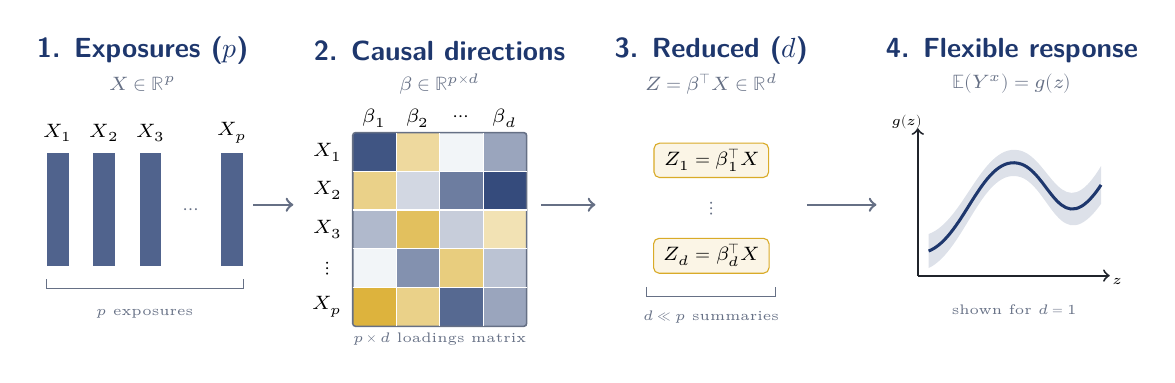
\begin{tikzpicture}[x=0.92cm,y=1.20cm]
  % Keep all stage titles and mathematical subtitles on shared baselines.
  \def\stageheadingy{2.92}
  \def\stagesubheadingy{2.57}

  % Stage headings and subtitles
  \uncover<2->{
  \node[font=\sffamily\bfseries\normalsize,text=emoryblue]
    at (1.35,\stageheadingy) {1. Exposures ($p$)};
  \node[font=\scriptsize,text=secondarygray] at (1.35,\stagesubheadingy)
    {$X\in\mathbb{R}^p$};
  }
  \uncover<3->{
  \node[font=\sffamily\bfseries\normalsize,text=emoryblue]
    at (5.45,\stageheadingy) {2. Causal directions};
  \node[font=\scriptsize,text=secondarygray] at (5.45,\stagesubheadingy)
    {$\beta\in\mathbb{R}^{p\times d}$};
  }
  \uncover<4->{
  \node[font=\sffamily\bfseries\normalsize,text=emoryblue]
    at (9.20,\stageheadingy) {3. Reduced ($d$)};
  \node[font=\scriptsize,text=secondarygray] at (9.20,\stagesubheadingy)
    {$Z=\beta^\top X\in\mathbb{R}^d$};
  }
  \uncover<5->{
  \node[font=\sffamily\bfseries\normalsize,text=emoryblue]
    at (13.35,\stageheadingy) {4. Flexible response};
  \node[font=\scriptsize,text=secondarygray] at (13.35,\stagesubheadingy)
    {$\mathbb{E}(Y^x)=g(z)$};
  }

  % 1. Exposure bars. A single color denotes a common object type;
  % no artificial ordering or exposure-level differences are implied.
  \uncover<2->{
  \fill[emoryblue!78!white] (0.03,0.64) rectangle ++(0.30,1.20);
  \fill[emoryblue!78!white] (0.67,0.64) rectangle ++(0.30,1.20);
  \fill[emoryblue!78!white] (1.31,0.64) rectangle ++(0.30,1.20);
  \fill[emoryblue!78!white] (2.43,0.64) rectangle ++(0.30,1.20);
  \node[font=\scriptsize,text=secondarygray] at (2.02,1.22) {$\cdots$};
  \node[font=\scriptsize] at (0.18,2.05) {$X_1$};
  \node[font=\scriptsize] at (0.82,2.05) {$X_2$};
  \node[font=\scriptsize] at (1.46,2.05) {$X_3$};
  \node[font=\scriptsize] at (2.58,2.05) {$X_p$};
  \draw[secondarygray,line width=0.45pt]
    (0.02,0.50) -- (0.02,0.40) -- (2.74,0.40) -- (2.74,0.50);
  \node[font=\tiny,text=secondarygray] at (1.38,0.14) {$p$ exposures};
  }

  % 2. Loading heatmap: columns are causal directions
  \uncover<3->{
  \begin{scope}[yshift=-0.14cm]
  \node[font=\scriptsize] at (4.55,2.32) {$\beta_1$};
  \node[font=\scriptsize] at (5.15,2.32) {$\beta_2$};
  \node[font=\scriptsize] at (5.75,2.32) {$\cdots$};
  \node[font=\scriptsize] at (6.35,2.32) {$\beta_d$};
  \node[font=\scriptsize] at (3.90,1.965) {$X_1$};
  \node[font=\scriptsize] at (3.90,1.555) {$X_2$};
  \node[font=\scriptsize] at (3.90,1.145) {$X_3$};
  \node[font=\scriptsize] at (3.90,0.735) {$\vdots$};
  \node[font=\scriptsize] at (3.90,0.325) {$X_p$};

  \fill[emoryblue!85!white] (4.25,1.76) rectangle ++(0.60,0.41);
  \fill[emorygold!45!white] (4.85,1.76) rectangle ++(0.60,0.41);
  \fill[lightpanel] (5.45,1.76) rectangle ++(0.60,0.41);
  \fill[emoryblue!45!white] (6.05,1.76) rectangle ++(0.60,0.41);
  \fill[emorygold!55!white] (4.25,1.35) rectangle ++(0.60,0.41);
  \fill[emoryblue!20!white] (4.85,1.35) rectangle ++(0.60,0.41);
  \fill[emoryblue!65!white] (5.45,1.35) rectangle ++(0.60,0.41);
  \fill[emoryblue!90!white] (6.05,1.35) rectangle ++(0.60,0.41);
  \fill[emoryblue!35!white] (4.25,0.94) rectangle ++(0.60,0.41);
  \fill[emorygold!75!white] (4.85,0.94) rectangle ++(0.60,0.41);
  \fill[emoryblue!25!white] (5.45,0.94) rectangle ++(0.60,0.41);
  \fill[emorygold!35!white] (6.05,0.94) rectangle ++(0.60,0.41);
  \fill[lightpanel] (4.25,0.53) rectangle ++(0.60,0.41);
  \fill[emoryblue!55!white] (4.85,0.53) rectangle ++(0.60,0.41);
  \fill[emorygold!60!white] (5.45,0.53) rectangle ++(0.60,0.41);
  \fill[emoryblue!30!white] (6.05,0.53) rectangle ++(0.60,0.41);
  \fill[emorygold!90!white] (4.25,0.12) rectangle ++(0.60,0.41);
  \fill[emorygold!55!white] (4.85,0.12) rectangle ++(0.60,0.41);
  \fill[emoryblue!75!white] (5.45,0.12) rectangle ++(0.60,0.41);
  \fill[emoryblue!45!white] (6.05,0.12) rectangle ++(0.60,0.41);
  \draw[secondarygray,line width=0.55pt,rounded corners=1pt]
    (4.25,0.12) rectangle (6.65,2.17);
  \foreach \x in {4.85,5.45,6.05}
    \draw[white,line width=0.45pt] (\x,0.12) -- (\x,2.17);
  \foreach \y in {0.53,0.94,1.35,1.76}
    \draw[white,line width=0.45pt] (4.25,\y) -- (6.65,\y);
  \node[font=\tiny,text=secondarygray] at (5.45,-0.02)
    {$p\times d$ loadings matrix};
  \end{scope}
  }

  % 3. Reduced causal scores
  \uncover<4->{
  \node[
    draw=emorygold,
    fill=softgold,
    rounded corners=2pt,
    inner xsep=0.13cm,
    inner ysep=0.08cm,
    font=\scriptsize
  ] at (9.20,1.76) {$Z_1=\beta_1^\top X$};
  \node[font=\scriptsize,text=secondarygray] at (9.20,1.25) {$\vdots$};
  \node[
    draw=emorygold,
    fill=softgold,
    rounded corners=2pt,
    inner xsep=0.13cm,
    inner ysep=0.08cm,
    font=\scriptsize
  ] at (9.20,0.75) {$Z_d=\beta_d^\top X$};
  \draw[secondarygray,line width=0.45pt]
    (8.31,0.42) -- (8.31,0.32) -- (10.09,0.32) -- (10.09,0.42);
  \node[font=\tiny,text=secondarygray] at (9.20,0.10) {$d\ll p$ summaries};
  }

  % 4. Flexible response curve
  \uncover<5->{
  \draw[->,textcharcoal,line width=0.70pt] (12.05,0.54) -- (14.70,0.54);
  \draw[->,textcharcoal,line width=0.70pt] (12.05,0.54) -- (12.05,2.10);
  \node[font=\tiny] at (14.80,0.48) {$z$};
  \node[font=\tiny] at (11.90,2.17) {$g(z)$};
  \fill[emoryblue!15!white]
    (12.20,0.98)
    .. controls (12.70,1.12) and (12.95,1.98) .. (13.48,1.86)
    .. controls (13.89,1.76) and (14.05,1.02) .. (14.58,1.70)
    -- (14.58,1.30)
    .. controls (14.02,0.70) and (13.88,1.46) .. (13.48,1.58)
    .. controls (12.95,1.72) and (12.70,0.80) .. (12.20,0.62)
    -- cycle;
  \draw[emoryblue,line width=1.10pt]
    (12.20,0.80)
    .. controls (12.70,0.95) and (12.95,1.86) .. (13.48,1.72)
    .. controls (13.88,1.61) and (14.03,0.86) .. (14.58,1.50);
  \node[font=\tiny,text=secondarygray] at (13.38,0.18) {shown for $d=1$};
  }

  % Flow arrows
  \uncover<3->{
  \draw[->,secondarygray,line width=0.90pt] (2.88,1.29) -- (3.43,1.29);
  }
  \uncover<4->{
  \draw[->,secondarygray,line width=0.90pt] (6.85,1.29) -- (7.60,1.29);
  }
  \uncover<5->{
  \draw[->,secondarygray,line width=0.90pt] (10.52,1.29) -- (11.48,1.29);
  }
\end{tikzpicture}
\end{center}

\vspace{0.34cm}

\begin{uncoverenv}<6->
\begin{center}
\underline{\textit{Question}}: How can we estimate $\mathcal{S}_{\mathbb{E}(Y^x)}$ when $\mathbb{E}(Y^x)=g(\beta^\top x)$?
\end{center}
\end{uncoverenv}
\end{frame}

\section{Estimation and Inference}\label{estimation-and-inference}

\begin{frame}{Marginal structural model approach}
\protect\phantomsection\label{marginal-structural-model-approach}
Using the theory of marginal structural models {\color{emoryblue}(Robins
2000)}, {\color{emoryblue}Nabi et al. (2022)} proposed estimating
\(\mathcal{S}_{\mathbb{E}(Y^x)}\) by solving the following efficient
score:

\[
\begin{aligned}
0={}&\frac{1}{n}\sum_{i=1}^n
\Bigg[
\frac{\pi^*(X_i)}{\pi(X_i\mid C_i)}
\Big\{Y_i-\mathbb E(Y\mid X_i,C_i)\Big\}
\\
&\quad\times
\Big\{\alpha(X_i)
-\mathbb E_q[\alpha(X)\mid\beta^\top X=\beta^\top X_i]\Big\}
\\[6pt]
&\quad+
\int_{\mathcal X}
\Big\{\mathbb E(Y\mid X=x,C_i)
-\mathbb E_q[Y\mid\beta^\top X=\beta^\top x]\Big\}
\\
&\quad\times
\Big\{\alpha(x)
-\mathbb E_q[\alpha(X)\mid\beta^\top X=\beta^\top x]\Big\}
\pi^*(x)\,dx
\Bigg].
\end{aligned}
\]
\end{frame}

\begin{frame}{Marginal structural model approach difficulties}
\protect\phantomsection\label{marginal-structural-model-approach-difficulties}
While the method is elegant, practical implementation is difficult.

\pause

Nuisance functions to be estimated:

\begin{enumerate}
\tightlist
\item
  \(m(x,c):= \mathbb{E}(Y\mid X, C)\)
\item
  \(\pi(x\mid c):= f_{X\mid C}(x\mid c)\)
\item
  \textcolor<3->{red}{$\mathbb{E}_q(Y\mid\beta^\top X=z)$}
\item
  \textcolor<3->{red}{$\mathbb{E}_q[\alpha(X)\mid\beta^\top X=z]$}
\end{enumerate}

\pause

\underline{\textit{Problem}}: Optimization is challenging when the
parameter is matrix-valued and nuisance functions must be re-estimated
at each iteration of \(\beta\).
\end{frame}

\begin{frame}{A simpler approach: recast the dose-response as a
regression}
\protect\phantomsection\label{a-simpler-approach-recast-the-dose-response-as-a-regression}
Suppose we can construct a variable \(\widetilde{Y}\) such that \[
\mathbb{E}(\widetilde{Y} \mid X=x) = \mathbb{E}(Y^x), \qquad \forall x\in \mathcal{X}.
\]

\pause

Then under our central assumption \(\mathbb{E}(Y^x)=g(\beta^\top x)\),
it follows that \[
\mathcal{S}_{\mathbb{E}(\widetilde{Y} \mid X)} = \mathcal{S}_{\mathbb{E}(Y^x)}. 
\]

\pause

\underline{\textit{Solution}}: Just run standard SDR for regression on
\((\widetilde{Y}, X)\) to estimate the causal
\(\mathcal{S}_{\mathbb{E}(Y^x)}\)!
\end{frame}

\begin{frame}{Estimation of \(\widetilde{Y}\)}
\protect\phantomsection\label{estimation-of-widetildey}
\begin{enumerate}
\tightlist
\item
  Causal dose-response: \[\widetilde{Y}=\mu(X).\]
\item
  Doubly robust pseudo-outcome: \[
  \widetilde{Y}=\xi=
  \frac{\pi(X)}{\pi(X\mid C)}
  \{Y-m(X,C)\}
  +\mathbb{E}_C[m(X,C)].
  \]
\end{enumerate}

Both require estimation of the same nuisances

\begin{itemize}
\tightlist
\item
  \(m(x,c)=\mathbb{E}(Y\mid X=x,C=c)\)
\item
  \(\pi(x\mid c)=f_{X\mid C}(x\mid c)\).
\end{itemize}
\end{frame}

\begin{frame}{Estimation of \(\mathcal{S}_{\mathbb{E}(Y\mid X)}\) with
MAVE}
\protect\phantomsection\label{estimation-of-mathcals_mathbbeymid-x-with-mave}
The minimum average variance estimator (MAVE) from {\color{emoryblue}Xia
et al. (2002)} estimates \(\mathcal{S}_{\mathbb{E}(Y\mid X)}\):
\begin{align*}
  \min_{\beta^\top\beta = I_d,\; \{a_j,{b}_j\}}
  \sum_{j=1}^n \sum_{i=1}^n 
  \Big(Y_i - \{a_j +   {b}_j^\top \beta^\top ({X}_i - {X}_j)\}\Big)^2 w_{ij}
\end{align*}

where \(w_{ij} = K_h(X_i-X_j) / \sum^n_{\ell=1} K_h(X_i - X_\ell)\).
\end{frame}

\begin{frame}{Our CSDR Approach}
\protect\phantomsection\label{our-csdr-approach}
\textbf{CSDR Algorithm} {\color{emoryblue}(Hsiao, Chang, et al. 2026)}:

\begin{enumerate}
\tightlist
\item
  Use \(O=(Y,X,C)\) to estimate \(\widetilde{Y}\).
\item
  Estimate \(\mathcal{S}_{\mathbb{E}(Y^x)}\) by running MAVE on
  \((\widetilde{Y}, X)\).
\item
  Estimate \(\mu(x)\) by replacing \(X\) with \(Z:=\hat{\beta}^\top X\).
  \[
  \widehat{\mu}_{DR,\widehat{\beta}}(z)
  =
  \frac{1}{n}\sum_{i=1}^n
  \left\{
  \frac{K_h(\widehat Z_i-z)}
  {\widehat{\pi}_{\widehat{\beta}}(\widehat Z_i\mid C_i)}
  \left[Y_i-\widehat m_{\widehat{\beta}}(\widehat Z_i,C_i)\right]
  +\widehat m_{\widehat{\beta}}(z,C_i)
  \right\},
  \]
\item
  Construct 95\% confidence intervals for
  \(\hat{\mu}_{DR, \hat{\beta}}(z)\) based on empirical variance of the
  influence function.
\end{enumerate}
\end{frame}

\begin{frame}{Alternative approach}
\protect\phantomsection\label{alternative-approach}
The CSDR approach improves on the MSM approach by avoiding numerical
optimization on \(\beta\)-dependent nuisances.

\vspace{0.4cm}

However, estimation of \(\widetilde{Y}\) still involves nuisance
estimation of \(m(x,c)\) and \(\pi(x\mid c)\).

\vspace{0.4cm}

We propose another alternative that can estimate
\(\mathcal{S}_{\mathbb{E}(Y^x)}\) without \(m(x,c)\) and
\(\pi(x\mid c)\).
\end{frame}

\begin{frame}{Partial dimension reduction on \(\mathbb{E}(Y\mid X,C)\)}
\protect\phantomsection\label{partial-dimension-reduction-on-mathbbeymid-xc}
For this approach, we make an additional assumption that \[
\mathbb{E}(Y^x \mid C=c) = g(\beta^\top x, c).
\] One can show that any \(\beta\) satisfying the above also satisfies
our original central assumption: \[
\mathbb{E}(Y^x) = g(\beta^\top x).
\] It follows that the partial central mean subspace of \(Y\) given
\((X, C)\) is equal to \(\mathcal{S}_{\mathbb{E}(Y^x)}\).

\pause

\vspace{0.34cm}

\underline{\textit{Solution}}: Run partial dimension reduction
{\color{emoryblue}(Li et al. 2010)} directly on
\(\mathbb{E}(Y\mid X,C)\).
\end{frame}

\begin{frame}{Theoretical results: subspace estimation}
\protect\phantomsection\label{theoretical-results-subspace-estimation}
Let \(\delta_n=\sqrt{{\log n} / ({nh^d})}\) and
\(\textcolor{red}{R_n}=\lVert \hat{\mu}(X)- \mu(X)\rVert_\infty\) (the
error in estimating \(\widetilde{Y}\)).

\pause

\vspace{0.34cm}

\begin{enumerate}
\tightlist
\item
  \textbf{Subspace estimation}: We establish convergence rates for
  estimating \(\mathcal{S}_{\mathbb{E}(Y^x)}\):
\end{enumerate}

\begin{itemize}
\tightlist
\item
  Method 1:
  \(\lVert \hat{\beta} - \beta\rVert = O_p(h^3+h\delta_n+h^{-1}\textcolor{red}{R_n})\)
  (dependent on \(\widetilde{Y}\) estimation)
\item
  Method 2:
  \(\lVert \hat{\beta} - \beta\rVert = O_p(h^3+h\delta_n+h^{-1}\delta_n^2)\)
  (nuisance estimation-free)
\end{itemize}

\pause

\vspace{0.34cm}

\begin{enumerate}
\setcounter{enumi}{1}
\tightlist
\item
  \textbf{Structural dimension selection}: A cross-validation procedure
  consistently estimates the dimension of
  \(\mathcal{S}_{\mathbb{E}(Y^x)}\). \[
  \mathbb{P}(\widehat d=d_0)\longrightarrow 1.
  \]
\end{enumerate}
\end{frame}

\begin{frame}{Theoretical results: asymptotic equivalence}
\protect\phantomsection\label{theoretical-results-asymptotic-equivalence}
One may wonder how estimating \(\mu(x)=\mathbb{E}(Y^x)\) using
\(\hat{\beta}_n\) compares to the true \(\beta\).

\pause

\textbf{Asymptotic equivalence}: We show that error in estimating
\(\beta\) can be \textit{asymptotically negligible} for estimating
\(\mu(x)\) {\color{emoryblue}(Forzani et al. 2024)}: \[
\sqrt{nh_n^d} \big\{ \hat{\mu}_{DR}({x}; \hat{\beta}_n) - \hat{\mu}_{DR}({x}; \beta) \big\} = o_p(1)
\]

\underline{\textit{Insight}}: Estimation of \(\beta\) can achieve
\(O_p(n^{-1/2})\) convergence, faster than the \(O_p\{(nh^d)^{-1/2}\}\)
rate of \(\hat{\mu}_{DR}(x)\).
\end{frame}

\begin{frame}{Theoretical results: subspace importance scores}
\protect\phantomsection\label{theoretical-results-subspace-importance-scores}
\underline{\textit{Problem}}: \(\beta\) is not uniquely identified, so
direct interpretation of loadings is tricky.

\underline{\textit{Solution}}: Measure each exposure's contribution
using the projection matrix, which is unique. \[
\boxed{\lambda_j = e_j^\top \beta(\beta^\top \beta)^{-1}\beta^\top e_j=\big[\beta(\beta^\top \beta)^{-1}\beta^\top\big]_{jj}}
\]

\begin{itemize}
\tightlist
\item
  Basis invariant: unaffected by rotations in \(\beta\).
\item
  Bounded: \(0\leq\lambda_j\leq 1\)
\item
  Decomposition: \(\sum_{j=1}^p\lambda_j=d\)
\end{itemize}
\end{frame}

\begin{frame}{Summary of our work}
\protect\phantomsection\label{summary-of-our-work}
Existing approaches either

\begin{itemize}
\tightlist
\item
  Estimated outcome regression instead of causal dose-response
\item
  Performed unsupervised dimension reduction that ignored causal
  structure
\item
  Conduct causal inference but on a scalar, joint shift exposure
\end{itemize}

\pause

Our approach builds on and combines the strengths of these previous
approaches

\begin{itemize}
\tightlist
\item
  Flexibly estimates the nonparametric dose-response in a lower
  dimension
\item
  Returns a causally and scientifically interpretable \(\beta\)
\item
  Final dose-response estimation is asymptotically robust to estimation
  error of \(\hat{\beta}\)
\end{itemize}
\end{frame}

\section{Simulations and Real Data}\label{simulations-and-real-data}

\begin{frame}{CSDR recovers the true \(\mathcal{S}_{\mathbb{E}(Y^x)}\)}
\protect\phantomsection\label{csdr-recovers-the-true-mathcals_mathbbeyx}
\begin{longtable}[]{@{}lrrr@{}}
\caption{Frobenius norm error between estimated and true
\(\mathcal{S}_{\mathbb{E}(Y^x)}\) with estimated \(\hat{d}\). Mean
(SD).}\label{tbl-error}\tabularnewline
\toprule\noalign{}
Method & \(n=500\) & \(n=1000\) & \(n=5000\) \\
\midrule\noalign{}
\endfirsthead
\toprule\noalign{}
Method & \(n=500\) & \(n=1000\) & \(n=5000\) \\
\midrule\noalign{}
\endhead
\textbf{CSDR} & 0.45 (0.39) & 0.22 (0.29) & 0.03 (0.04) \\
pCCA & 1.20 (0.18) & 1.10 (0.20) & 0.74 (0.20) \\
MAVE & 1.29 (0.17) & 1.17 (0.10) & 1.07 (0.02) \\
PCA & 2.00 (0.00) & 2.00 (0.00) & 2.00 (0.00) \\
\bottomrule\noalign{}
\end{longtable}
\end{frame}

\begin{frame}{CSDR recovers the true structural dimension}
\protect\phantomsection\label{csdr-recovers-the-true-structural-dimension}
\begin{longtable}[]{@{}llrrrr@{}}
\caption{Proportion selecting each dimension
(\(d_0=2\)).}\label{tbl-dimension}\tabularnewline
\toprule\noalign{}
\(n\) & Method & \(d=1\) & \(d=2\) & \(d=3\) & \(d=4\) \\
\midrule\noalign{}
\endfirsthead
\toprule\noalign{}
\(n\) & Method & \(d=1\) & \(d=2\) & \(d=3\) & \(d=4\) \\
\midrule\noalign{}
\endhead
500 & \textbf{CSDR} & 0.03 & \textbf{0.88} & 0.07 & 0.01 \\
& MAVE & 0.00 & \textbf{0.11} & 0.75 & 0.14 \\
5000 & \textbf{CSDR} & 0.00 & \textbf{1.00} & 0.00 & 0.00 \\
& MAVE & 0.00 & \textbf{0.00} & 1.00 & 0.00 \\
\bottomrule\noalign{}
\end{longtable}
\end{frame}

\begin{frame}{CSDR improves inference of the causal dose-response}
\protect\phantomsection\label{csdr-improves-inference-of-the-causal-dose-response}
\begin{figure}

\centering{

\includegraphics[width=0.7\linewidth,height=\textheight,keepaspectratio]{../../results/jasa-initial-submission/main_paper_final_results_nnet/interaction/Simulation_Coverage.png}

}

\caption{\label{fig-simulation-coverage}Pointwise 95\% coverage for the
exposure-response curve (\(p=10\), \(d=2\)) at \(100\) test points;
methods differ only in \(\beta\) estimation.}

\end{figure}%
\end{frame}

\begin{frame}{PFAS real data application}
\protect\phantomsection\label{pfas-real-data-application}
\newcommand{\pfasStudyCitation}{{\color{emoryblue}(Chang et al. 2022)}}

\begin{columns}[T]
\begin{column}{0.39\linewidth}
\centering
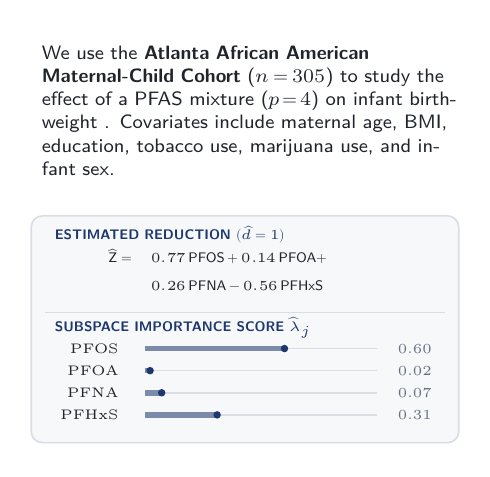
\begin{tikzpicture}[x=0.46cm,y=0.72cm]
  \path[use as bounding box] (0,0) rectangle (12.00,7.42);

  % Study setup
  \node[
    anchor=north west,
    text width=5.30cm,
    align=left,
    font=\sffamily\fontsize{7.0}{8.4}\selectfont,
    text=textcharcoal
  ] at (0.12,7.28) {We use the \textbf{Atlanta African American
  Maternal-Child Cohort} (\(n\!=\!305\)) to study the effect of a PFAS
  mixture (\(p\!=\!4\)) on infant birthweight \pfasStudyCitation. Covariates include maternal
  age, BMI, education, tobacco use, marijuana use, and infant sex.};

  % Estimated results
  \filldraw[
    fill=lightpanel!68!white,
    draw=rulegray,
    line width=0.60pt,
    rounded corners=4pt
  ] (0.10,0.10) rectangle (11.90,4.10);

  % Estimated summary
  \node[
    anchor=west,
    font=\sffamily\bfseries\tiny,
    text=emoryblue
  ] at (0.48,3.77) {ESTIMATED REDUCTION \((\widehat d=1)\)};
  \node[
    font=\sffamily\tiny,
    text=textcharcoal,
    anchor=base east
  ] at (3.15,3.28) {\(\widehat{\mathsf{Z}}=\)};
  \node[
    font=\sffamily\tiny,
    text=textcharcoal,
    anchor=base west
  ] at (3.15,3.28)
    {\(0.77\,\text{PFOS}+0.14\,\text{PFOA}+\)};
  \node[
    font=\sffamily\tiny,
    text=textcharcoal,
    anchor=base west
  ] at (3.15,2.79)
    {\(0.26\,\text{PFNA}-0.56\,\text{PFHxS}\)};
  \draw[rulegray,line width=0.45pt] (0.48,2.40) -- (11.52,2.40);

  % SIS lollipop report
  \node[
    anchor=west,
    font=\sffamily\bfseries\tiny,
    text=emoryblue
  ] at (0.48,2.12) {SUBSPACE IMPORTANCE SCORE \(\widehat\lambda_j\)};

  \foreach \y in {1.76,1.37,0.98,0.59} {
    \draw[rulegray,line width=0.55pt] (3.25,\y) -- (9.65,\y);
  }
  \node[font=\tiny,text=textcharcoal,anchor=east] at (2.78,1.76) {PFOS};
  \node[font=\tiny,text=textcharcoal,anchor=east] at (2.78,1.37) {PFOA};
  \node[font=\tiny,text=textcharcoal,anchor=east] at (2.78,0.98) {PFNA};
  \node[font=\tiny,text=textcharcoal,anchor=east] at (2.78,0.59) {PFHxS};

  \draw[emoryblue!58!white,line width=2.00pt] (3.25,1.76) -- (7.09,1.76);
  \fill[emoryblue] (7.09,1.76) circle[radius=1.35pt];
  \node[font=\tiny,text=secondarygray,anchor=west] at (9.95,1.76) {0.60};

  \draw[emoryblue!58!white,line width=2.00pt] (3.25,1.37) -- (3.38,1.37);
  \fill[emoryblue] (3.38,1.37) circle[radius=1.35pt];
  \node[font=\tiny,text=secondarygray,anchor=west] at (9.95,1.37) {0.02};

  \draw[emoryblue!58!white,line width=2.00pt] (3.25,0.98) -- (3.70,0.98);
  \fill[emoryblue] (3.70,0.98) circle[radius=1.35pt];
  \node[font=\tiny,text=secondarygray,anchor=west] at (9.95,0.98) {0.07};

  \draw[emoryblue!58!white,line width=2.00pt] (3.25,0.59) -- (5.23,0.59);
  \fill[emoryblue] (5.23,0.59) circle[radius=1.35pt];
  \node[font=\tiny,text=secondarygray,anchor=west] at (9.95,0.59) {0.31};
\end{tikzpicture}
\end{column}

\begin{column}{0.58\linewidth}
\begingroup
\captionsetup{font=pfasapplication}

\begin{figure}[H]

{\centering \includegraphics[width=0.9\linewidth,height=\textheight,keepaspectratio]{../../results/jasa-initial-submission/ATL-AA/ers_causal_no_title_main_paper.pdf}

}

\caption{PFAS exposure-response curve from ATL-AA}

\end{figure}%

\endgroup
\end{column}
\end{columns}
\end{frame}

\begin{frame}{BKMR and qgcomp comparison analysis}
\protect\phantomsection\label{bkmr-and-qgcomp-comparison-analysis}
\vspace{-0.10cm}
\begin{columns}[T,onlytextwidth]
\begin{column}{0.465\linewidth}
\begin{block}{BKMR}
\begin{minipage}[t][4.55cm][t]{\linewidth}
\begin{minipage}[c][3.75cm][c]{\linewidth}
\centering
\includegraphics[
  width=0.96\linewidth,
  height=3.45cm,
  keepaspectratio
]{../../results/jasa-initial-submission/ATL-AA/bkmr_diff.pdf}
\end{minipage}

\vspace{0.04cm}

\begin{minipage}[c][0.52cm][c]{\linewidth}
\centering
{\scriptsize\color{secondarygray}
All four PFAS share a quantile versus the median.}
\end{minipage}
\end{minipage}
\end{block}
\end{column}

\hfill

\begin{column}{0.465\linewidth}
\begin{block}{qgcomp}
\begin{minipage}[t][4.55cm][t]{\linewidth}
\begin{minipage}[c][3.75cm][c]{\linewidth}
\centering
\includegraphics[
  width=0.96\linewidth,
  height=3.45cm,
  keepaspectratio
]{../../results/jasa-initial-submission/ATL-AA/qgcomp.pdf}
\end{minipage}

\vspace{0.04cm}

\begin{minipage}[c][0.52cm][c]{\linewidth}
\centering
{\scriptsize\color{secondarygray}
All four PFAS shift together across exposure quartiles.}
\end{minipage}
\end{minipage}
\end{block}
\end{column}
\end{columns}

\vspace{0.12cm}

\begin{center}
\scriptsize
\method{Takeaway:} Different estimands, but in general, increasing PFAS leads to
decreasing birthweight.
\end{center}
\end{frame}

\section{Future Directions}\label{future-directions}

\begin{frame}{Causal dimension reduction for mediation analysis}
\protect\phantomsection\label{causal-dimension-reduction-for-mediation-analysis}
Colleagues in EH want to study biological mechanisms of exposures using
omics.

Can CSDR ideas preserve mediation effects and identify important
mediators in \(M\)? \vspace{0.34cm}

\vspace{0.10cm}
\begin{columns}[T,onlytextwidth]
\begin{column}{0.49\textwidth}
\centering
\method{Reduction between $X$ and $M$}\\[0.12cm]
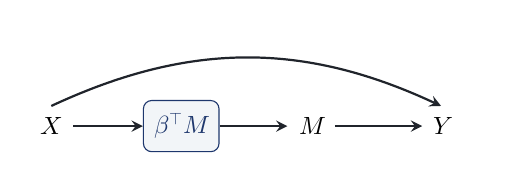
\begin{tikzpicture}[
  x=1cm,y=1cm,
  every node/.style={font=\small,inner sep=4pt},
  reduced/.style={draw=emoryblue,fill=lightpanel,rounded corners=3pt,
    text=emoryblue,minimum height=0.65cm},
  edge/.style={->,>=stealth,thick,draw=textcharcoal}
]
  \path[use as bounding box] (-0.3,-0.45) rectangle (5.5,1.25);
  \node (x) at (0.0,0) {$X$};
  \node[reduced] (b) at (1.65,0) {$\beta^\top M$};
  \node (m) at (3.3,0) {$M$};
  \node (y) at (4.949999999999999,0) {$Y$};
  \draw[edge] (x) -- (b);
  \draw[edge] (b) -- (m);
  \draw[edge] (m) -- (y);
  \draw[edge] (x.north) to[bend left=25] (y.north);
\end{tikzpicture}
\end{column}
\begin{column}{0.49\textwidth}
\centering
\method{Reduction between $M$ and $Y$}\\[0.12cm]
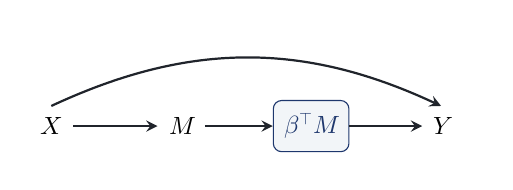
\begin{tikzpicture}[
  x=1cm,y=1cm,
  every node/.style={font=\small,inner sep=4pt},
  reduced/.style={draw=emoryblue,fill=lightpanel,rounded corners=3pt,
    text=emoryblue,minimum height=0.65cm},
  edge/.style={->,>=stealth,thick,draw=textcharcoal}
]
  \path[use as bounding box] (-0.3,-0.45) rectangle (5.5,1.25);
  \node (x) at (0.0,0) {$X$};
  \node (m) at (1.65,0) {$M$};
  \node[reduced] (b) at (3.3,0) {$\beta^\top M$};
  \node (y) at (4.949999999999999,0) {$Y$};
  \draw[edge] (x) -- (m);
  \draw[edge] (m) -- (b);
  \draw[edge] (b) -- (y);
  \draw[edge] (x.north) to[bend left=25] (y.north);
\end{tikzpicture}
\end{column}
\end{columns}
\begin{center}
\scriptsize\textcolor{secondarygray}{Confounders $C$ omitted for clarity.}
\end{center}
\vspace{-0.15cm}

\vspace{0.34cm}

\underline{\textit{Problem}}: Preserving the mediation effect alone may
not capture both the exposure--mediator and mediator--outcome
relationships.
\end{frame}

\begin{frame}{Causal representation learning}
\protect\phantomsection\label{causal-representation-learning}
Can we extend CSDR from linear subspaces to \textbf{nonlinear,
interpretable representations}?

Variational autoencoders offer a template.

\begin{center}
\usetikzlibrary{shapes.geometric}
\begin{tikzpicture}[
  x=1cm,y=1cm,
  every node/.style={font=\scriptsize,align=center},
  vaebox/.style={draw=rulegray,fill=lightpanel,rounded corners=3pt,
    minimum width=1.85cm,minimum height=1.05cm},
  edge/.style={->,>=stealth,thick,draw=emoryblue}
]
  \path[use as bounding box] (-1.05,-2.1) rectangle (11.5,0.95);
  \node[vaebox] (input) at (0,0) {Original variables\\[0.08cm]$V=X$ or $M$};
  \node[draw=emoryblue,fill=emoryblue!10,trapezium,
    trapezium left angle=75,trapezium right angle=105,
    minimum width=1.65cm,minimum height=1.15cm] (encoder) at (2.55,0)
    {\textbf{Encoder}\\$q_\phi(Z\mid V)$};
  \node[vaebox,draw=emoryblue,text=emoryblue] (latent) at (5.1,0)
    {Latent sample\\[0.08cm]$Z\sim q_\phi(Z\mid V)$};
  \node[draw=emoryblue,fill=emoryblue!10,trapezium,
    trapezium left angle=105,trapezium right angle=75,
    minimum width=1.65cm,minimum height=1.15cm] (decoder) at (7.65,0)
    {\textbf{Decoder}\\$p_\theta(V\mid Z)$};
  \node[vaebox] (output) at (10.2,0)
    {Reconstruction\\[0.08cm]$\widetilde V$};
  \draw[edge] (input) -- (encoder);
  \draw[edge] (encoder) -- (latent);
  \draw[edge] (latent) -- (decoder);
  \draw[edge] (decoder) -- (output);
  \node[draw=emorygolddark,fill=softgold,rounded corners=3pt,
    text=emorygolddark,minimum width=4.5cm,minimum height=0.72cm]
    (causal) at (5.1,-1.65)
    {\textbf{Proposed causal objective}\\Preserve the causal estimand};
  \draw[edge,draw=emorygolddark] (latent) -- (causal);
\end{tikzpicture}
\end{center}

\underline{\textit{Why I am excited}}: could help address many common
problems in biomarker discovery including curse of dimensionality,
positivity violations, and interpretability.
\end{frame}

\begin{frame}{Data fusion for improved health surveillance}
\protect\phantomsection\label{data-fusion-for-improved-health-surveillance}
In previous work {\color{emoryblue}(Hsiao et al. 2025; Hsiao, Fede, et
al. 2026; Varghese et al. 2026)}, we estimated county-level hypertension
care cascade comparing

\begin{itemize}
\tightlist
\item
  NHANES (national, probability)
\item
  BRFSS survey data (county, probability)
\item
  Self-service kiosk data (county, nonprobability)
\item
  Epic COSMOS EHR (county, nonprobability)
\end{itemize}

\underline{\textit{Problem}}: Can we combine NHANES and large
nonprobability samples (e.g., kiosks, EHR) in an intelligent way? Can
spatiotemporal dependence further improve estimates?
\end{frame}

\begin{frame}{Final thoughts}
\protect\phantomsection\label{final-thoughts}
What I bring

\begin{itemize}
\tightlist
\item
  Causal inference, dimension reduction, spatiotemporal statistics
\item
  Applications in environmental health, EHR, disease surveillance for
  public health impact
\item
  Engagement and leadership in scientific collaborations, teaching, and
  mentorship
\end{itemize}

\vspace{0.15cm}

I would love to build this agenda at Wake Forest and contribute to its
growing research community. I am especially excited about opportunities
across the School of Medicine, Advocate Health, and Statistical
Sciences.
\end{frame}

\begin{frame}[allowframebreaks]{References}
\protect\phantomsection\label{references}
\fontsize{6}{6.5}\selectfont
\setbeamerfont{bibliography entry author}{size=\fontsize{6}{6.5}}
\renewenvironment{CSLReferences}[2]
  {\begin{list}{}{%
    \setlength{\leftmargin}{1em}%
    \setlength{\itemindent}{-1em}%
    \setlength{\parsep}{0pt}%
    \setlength{\itemsep}{0pt}%
    \setlength{\topsep}{0pt}}%
    \fontsize{6}{6.5}\selectfont}
  {\end{list}}

\protect\phantomsection\label{refs}
\begin{CSLReferences}{1}{1}
\bibitem[\citeproctext]{ref-bobbBayesianKernelMachine2015}
Bobb, Jennifer F., Linda Valeri, Birgit Claus Henn, et al. 2015.
{``Bayesian Kernel Machine Regression for Estimating the Health Effects
of Multi-Pollutant Mixtures.''} \emph{Biostatistics} 16 (3): 493--508.

\bibitem[\citeproctext]{ref-changPolyfluoroalkylSubstancePFAS2022}
Chang, Che-Jung, Dana Boyd Barr, P.Barry Ryan, et al. 2022. {``Per- and
Polyfluoroalkyl Substance ({PFAS}) Exposure, Maternal Metabolomic
Perturbation, and Fetal Growth in {African American} Women: {A}
Meet-in-the-Middle Approach.''} \emph{Environment International} 158
(January): 106964.

\bibitem[\citeproctext]{ref-colangeloDoubleDebiasedMachine2026}
Colangelo, Kyle, and Ying-Ying Lee. 2026. {``Double {Debiased Machine
Learning Nonparametric Inference} with {Continuous Treatments}.''}
\emph{Journal of Business \& Economic Statistics} 44 (1): 67--79.

\bibitem[\citeproctext]{ref-cookFoundationalArgumentsSufficient2026}
Cook, R. Dennis. 2026. {``On the {Foundational Arguments} of {Sufficient
Dimension Reduction}.''} \emph{WIREs Computational Statistics} 18 (2):
e70064.

\bibitem[\citeproctext]{ref-forzaniAsymptoticResultsNonparametric2024}
Forzani, Liliana, Daniela Rodriguez, and Mariela Sued. 2024.
{``Asymptotic Results for Nonparametric Regression Estimators After
Sufficient Dimension Reduction Estimation.''} \emph{TEST} 33 (4):
987--1013.

\bibitem[\citeproctext]{ref-gibsonPrincipalComponentPursuit2022}
Gibson, Elizabeth A., Junhui Zhang, Jingkai Yan, et al. 2022.
{``Principal {Component Pursuit} for {Pattern Identification} in
{Environmental Mixtures}.''} \emph{Environmental Health Perspectives}
130 (11): 117008.

\bibitem[\citeproctext]{ref-hsiaoCausalSufficientDimension2026}
Hsiao, Thomas W., Howard H. Chang, and Razieh Nabi. 2026. \emph{Causal
{Sufficient Dimension Reduction} for {Multiple Continuous Exposures}
with an {Application} to {Environmental Mixtures}}. arXiv:2606.14840.
arXiv.

\bibitem[\citeproctext]{ref-hsiaoCountyPrevalenceAwareness2026}
Hsiao, Thomas W., Lauren Fede, Cameron Gocke, Lance A. Waller, Mohammed
K. Ali, and Jithin Sam Varghese. 2026. {``County {Prevalence},
{Awareness}, and {Control} of {High Blood Pressure From Health Kiosks}
in the {United States}, 2017--2024.''} \emph{Hypertension} 83 (2):
e25829.

\bibitem[\citeproctext]{ref-hsiaoBloodPressureMeasurements2025}
Hsiao, Thomas W., Jithin Sam Varghese, Lauren Fede, Cameron Gocke, Lance
A. Waller, and Mohammed K. Ali. 2025. {``Blood {Pressure Measurements
From Self-Service Health Kiosks} in {US Retail Stores}, 2017-2024.''}
\emph{JAMA Cardiology} 10 (10): 1044--48.

\bibitem[\citeproctext]{ref-keilQuantileBasedGComputationApproach2020}
Keil, Alexander P., Jessie P. Buckley, Katie M. O'Brien, Kelly K.
Ferguson, Shanshan Zhao, and Alexandra J. White. 2020. {``A
{Quantile-Based} g-{Computation Approach} to {Addressing} the {Effects}
of {Exposure Mixtures}.''} \emph{Environmental Health Perspectives} 128
(4): 047004.

\bibitem[\citeproctext]{ref-liGroupwiseDimensionReduction2010}
Li, Lexin, Bing Li, and Li-Xing Zhu. 2010. {``Groupwise {Dimension
Reduction}.''} \emph{Journal of the American Statistical Association}
105 (491): 1188--201.

\bibitem[\citeproctext]{ref-nabiSemiparametricCausalSufficient2022}
Nabi, Razieh, Todd McNutt, and Ilya Shpitser. 2022. {``Semiparametric
Causal Sufficient Dimension Reduction of Multidimensional Treatments.''}
\emph{Proceedings of the {Thirty-Eighth Conference} on {Uncertainty} in
{Artificial Intelligence}}, August, 1445--55.

\bibitem[\citeproctext]{ref-robinsMarginalStructuralModels2000a}
Robins, James M. 2000. {``Marginal {Structural Models} Versus
{Structural} Nested {Models} as {Tools} for {Causal} Inference.''} In
\emph{Statistical {Models} in {Epidemiology}, the {Environment}, and
{Clinical Trials}}, edited by Willard Miller, M. Elizabeth Halloran, and
Donald Berry, vol. 116. Springer New York.

\bibitem[\citeproctext]{ref-vargheseNationalStateCounty2026a}
Varghese, Jithin Sam, Thomas W. Hsiao, Lauren Fede, et al. 2026.
{``National, {State}, and {County Estimates} of {Adult Overweight} and
{Obesity From Electronic Health Records} and {Kiosks} in {Retail
Locations}, 2024--2025.''} \emph{Obesity} 34 (4): 908--16.

\bibitem[\citeproctext]{ref-xiaAdaptiveEstimationDimension2002}
Xia, Yingcun, Howell Tong, W. K. Li, and Li-Xing Zhu. 2002. {``An
{Adaptive Estimation} of {Dimension Reduction Space}.''} \emph{Journal
of the Royal Statistical Society. Series B (Statistical Methodology)} 64
(3): 363--410.

\end{CSLReferences}
\end{frame}

\begin{frame}{Acknowledgments}
\protect\phantomsection\label{acknowledgments}
\centering
\large

\method{Postdoctoral advisors}\\[0.16cm]
\textbf{Howard Chang}
\hspace{0.28cm}\raisebox{-0.08cm}{\color{emorygold}\rule{0.8pt}{0.38cm}}\hspace{0.28cm}
\textbf{Razieh Nabi}\\[0.12cm]
\small For their mentorship, guidance, and support.

\vspace{0.36cm}
{\color{rulegray}\rule{0.72\linewidth}{0.6pt}}
\vspace{0.32cm}

\large
\method{Collaborators}\\[0.16cm]
\textbf{Anne Dunlop}
\hspace{0.18cm}\raisebox{-0.08cm}{\color{emorygold}\rule{0.8pt}{0.38cm}}\hspace{0.18cm}
\textbf{Stephanie Eick}
\hspace{0.18cm}\raisebox{-0.08cm}{\color{emorygold}\rule{0.8pt}{0.38cm}}\hspace{0.18cm}
\textbf{Donghai Liang}
\hspace{0.18cm}\raisebox{-0.08cm}{\color{emorygold}\rule{0.8pt}{0.38cm}}\hspace{0.18cm}
\textbf{Youran Tan}\\[0.14cm]
\small For sharing the ATL-AA cohort data and for their thoughtful discussions.
\end{frame}

\begin{frame}{Questions?}
\protect\phantomsection\label{questions}
\centering
\vspace{0.18cm}

\begin{columns}[T,onlytextwidth]
\begin{column}{0.46\textwidth}
\centering
\href{https://arxiv.org/abs/2606.14840}{%
  
\includegraphics[height=0.72cm]{assets/arxiv-logo.png}}\\[0.13cm]
\href{https://arxiv.org/abs/2606.14840}{%
  
\includegraphics[width=3.05cm]{assets/qr-arxiv.png}}\\[0.10cm]
\textbf{CSDR preprint}\\[-0.01cm]
\href{https://arxiv.org/abs/2606.14840}{%
  \scriptsize\texttt{arxiv.org/abs/2606.14840}}
\end{column}

\begin{column}{0.46\textwidth}
\centering
\href{https://github.com/tXiao95/csdr}{%
  
\includegraphics[height=0.72cm]{assets/github-invertocat.png}}\\[0.13cm]
\href{https://github.com/tXiao95/csdr}{%
  
\includegraphics[width=3.05cm]{assets/qr-github.png}}\\[0.10cm]
\textbf{\texttt{csdr} R package}\\[-0.01cm]
\href{https://github.com/tXiao95/csdr}{%
  \scriptsize\texttt{github.com/tXiao95/csdr}}
\end{column}
\end{columns}

\csdrrecordappendixboundary
\end{frame}

\section{Appendix}\label{appendix}

\begin{frame}[fragile,t]{Setup outcome, exposures, and confounders}
\protect\phantomsection\label{setup-outcome-exposures-and-confounders}
\begin{columns}[T]
\begin{column}{0.4\linewidth}
\method{R code}

\workflowcodefont

\begin{Shaded}
\begin{Highlighting}[]
\FunctionTok{library}\NormalTok{(csdr)}
\FunctionTok{data}\NormalTok{(csdr\_example2)}

\NormalTok{Y }\OtherTok{\textless{}{-}}\NormalTok{ csdr\_example2}\SpecialCharTok{$}\NormalTok{Y}
\NormalTok{A }\OtherTok{\textless{}{-}}\NormalTok{ csdr\_example2}\SpecialCharTok{$}\NormalTok{A}
\NormalTok{C }\OtherTok{\textless{}{-}}\NormalTok{ csdr\_example2}\SpecialCharTok{$}\NormalTok{C}

\FunctionTok{head}\NormalTok{(Y, }\DecValTok{5}\NormalTok{)}
\FunctionTok{head}\NormalTok{(A[, }\FunctionTok{c}\NormalTok{(}\DecValTok{1}\SpecialCharTok{:}\DecValTok{3}\NormalTok{, }\DecValTok{18}\SpecialCharTok{:}\DecValTok{20}\NormalTok{)], }\DecValTok{5}\NormalTok{)}
\FunctionTok{head}\NormalTok{(C, }\DecValTok{5}\NormalTok{)}
\end{Highlighting}
\end{Shaded}
\end{column}

\begin{column}{0.56\linewidth}
\method{Console}

\workflowcodefont

\begin{Shaded}
\begin{Highlighting}[]
\NormalTok{\textgreater{} head(Y, 5)}
\NormalTok{     obs1      obs2      obs3      obs4      obs5}
\NormalTok{  0.3805    0.1838   {-}2.0486    0.4977    5.4798}

\NormalTok{\textgreater{} head(A[, c(1:3, 18:20)], 5)}
\NormalTok{         A1     A2     A3    A18    A19    A20}
\NormalTok{obs1 {-}1.066  1.573  0.953  0.033 {-}0.480  0.500}
\NormalTok{obs2 {-}1.028  0.325 {-}0.364 {-}0.967 {-}1.543 {-}0.572}
\NormalTok{obs3 {-}0.800 {-}0.103 {-}0.433 {-}0.011  0.505  0.623}
\NormalTok{obs4  2.492  0.582 {-}1.134 {-}1.473 {-}1.138  1.551}
\NormalTok{obs5  1.733 {-}0.114  0.615  1.083  0.350  0.133}

\NormalTok{\textgreater{} head(C, 5)}
\NormalTok{         C1    C2     C3     C4     C5}
\NormalTok{obs1 {-}0.935 1.312 {-}0.294 {-}1.979  1.150}
\NormalTok{obs2 {-}0.694 0.531  0.367 {-}2.259 {-}1.293}
\NormalTok{obs3 {-}0.548 0.712 {-}0.088 {-}0.407  1.828}
\NormalTok{obs4  0.766 1.050 {-}0.498 {-}0.593 {-}0.604}
\NormalTok{obs5  1.852 {-}0.554  0.849  0.643 {-}0.312}
\end{Highlighting}
\end{Shaded}
\end{column}
\end{columns}
\end{frame}

\begin{frame}[fragile,t]{Fit the causal subspace}
\protect\phantomsection\label{fit-the-causal-subspace}
\begin{columns}[T]
\begin{column}{0.4\linewidth}
\method{R code}

\workflowcodefont

\begin{Shaded}
\begin{Highlighting}[]
\NormalTok{sl\_lib }\OtherTok{\textless{}{-}} \FunctionTok{c}\NormalTok{(}
  \StringTok{"SL.glm"}\NormalTok{, }\StringTok{"SL.earth"}\NormalTok{, }\StringTok{"SL.ranger"}
\NormalTok{)}

\NormalTok{learners }\OtherTok{\textless{}{-}} \FunctionTok{csdr\_learners}\NormalTok{(}
  \AttributeTok{sl\_library =}\NormalTok{ sl\_lib}
\NormalTok{)}

\FunctionTok{set.seed}\NormalTok{(}\DecValTok{42}\NormalTok{)}
\NormalTok{fit }\OtherTok{\textless{}{-}} \FunctionTok{csdr}\NormalTok{(}
  \AttributeTok{Y =}\NormalTok{ Y, }\AttributeTok{A =}\NormalTok{ A, }\AttributeTok{C =}\NormalTok{ C,}
  \AttributeTok{L =} \DecValTok{5}\NormalTok{, }\AttributeTok{seed =} \DecValTok{42}\NormalTok{,}
  \AttributeTok{learners =}\NormalTok{ learners,}
  \AttributeTok{max\_dim =} \DecValTok{5}\NormalTok{,}
  \AttributeTok{keep\_nuisance =} \ConstantTok{TRUE}
\NormalTok{)}

\FunctionTok{summary}\NormalTok{(fit)}
\end{Highlighting}
\end{Shaded}
\end{column}

\begin{column}{0.56\linewidth}
\method{Console}

\workflowcodefont

\begin{Shaded}
\begin{Highlighting}[]
\NormalTok{\textgreater{} summary(fit)}
\NormalTok{Summary of causal sufficient dimension reduction fit}

\NormalTok{ variant d\_hat  n p mave\_method target\_exposure}
\NormalTok{      DR     2 100 20   meanMAVE               A}

\NormalTok{Learners:}
\NormalTok{ outcome: SuperLearner regression}
\NormalTok{   family: gaussian}
\NormalTok{   SL.library: SL.glm, SL.earth, SL.ranger}
\NormalTok{ gps: MVN GPS with linear conditional mean}
\NormalTok{   method\_gps: linear; density\_floor: 1e{-}16}

\NormalTok{Target construction:}
\NormalTok{Effective folds: 5}
\NormalTok{PO marginalization: crossfit}
\end{Highlighting}
\end{Shaded}
\end{column}
\end{columns}
\end{frame}

\begin{frame}[fragile,t]{Inspect the fitted subspace and scores}
\protect\phantomsection\label{inspect-the-fitted-subspace-and-scores}
\begin{columns}[T]
\begin{column}{0.4\linewidth}
\method{R code}

\workflowcodefont

\begin{Shaded}
\begin{Highlighting}[]
\NormalTok{B\_hat }\OtherTok{\textless{}{-}} \FunctionTok{coef}\NormalTok{(fit)}
\NormalTok{Z\_hat }\OtherTok{\textless{}{-}} \FunctionTok{scores}\NormalTok{(fit)}

\NormalTok{mave }\OtherTok{\textless{}{-}} \FunctionTok{mave\_fits}\NormalTok{(fit)}
\NormalTok{dim\_selection }\OtherTok{\textless{}{-}}\NormalTok{ mave}\SpecialCharTok{$}\NormalTok{dimension\_selection}

\NormalTok{B\_hat[}\FunctionTok{c}\NormalTok{(}\DecValTok{1}\NormalTok{, }\DecValTok{2}\NormalTok{, }\DecValTok{20}\NormalTok{), , drop }\OtherTok{=} \ConstantTok{FALSE}\NormalTok{]}
\FunctionTok{sis}\NormalTok{(fit)}
\FunctionTok{head}\NormalTok{(Z\_hat, }\DecValTok{2}\NormalTok{)}
\NormalTok{dim\_selection}
\end{Highlighting}
\end{Shaded}
\end{column}

\begin{column}{0.56\linewidth}
\method{Console}

\workflowcodefont

\begin{Shaded}
\begin{Highlighting}[]
\NormalTok{\textgreater{} B\_hat[c(1, 2, 20), , drop = FALSE]}
\NormalTok{       dir1    dir2}
\NormalTok{A1 {-}0.3401  0.5777}
\NormalTok{A2 {-}0.3524  0.4195}
\NormalTok{A20 {-}0.0521 0.0784}

\NormalTok{\textgreater{} sis(fit)}
\NormalTok{    A1    A2    A3    A4    A5    A6    A7    A8    A9   A10}
\NormalTok{ 0.464 0.312 0.533 0.390 0.000 0.004 0.002 0.020 0.001 0.021}
\NormalTok{   A11   A12   A13   A14   A15   A16   A17   A18   A19   A20}
\NormalTok{ 0.068 0.059 0.028 0.020 0.006 0.005 0.015 0.036 0.006 0.009}

\NormalTok{\textgreater{} head(Z\_hat, 2)}
\NormalTok{       score1  score2}
\NormalTok{obs1  {-}0.1862  0.4515}
\NormalTok{obs2   1.5224 {-}0.3484}

\NormalTok{\textgreater{} dim\_selection}
\NormalTok{Dimensions      0    1    2    3    4    5}
\NormalTok{CV{-}value     1.58 1.13 0.75 0.77 0.92 0.97}
\NormalTok{Selected dimension: 2}
\end{Highlighting}
\end{Shaded}
\end{column}
\end{columns}
\end{frame}

\begin{frame}[fragile,t]{Estimate the response in the reduced exposure}
\protect\phantomsection\label{estimate-the-response-in-the-reduced-exposure}
\begin{columns}[T]
\begin{column}{0.4\linewidth}
\method{R code}

\workflowcodefont

\begin{Shaded}
\begin{Highlighting}[]
\NormalTok{z\_grid }\OtherTok{\textless{}{-}} \FunctionTok{matrix}\NormalTok{(}
  \FunctionTok{rep}\NormalTok{(}\FunctionTok{apply}\NormalTok{(Z\_hat, }\DecValTok{2}\NormalTok{, median), }\AttributeTok{each =} \DecValTok{50}\NormalTok{),}
  \AttributeTok{nrow =} \DecValTok{50}\NormalTok{,}
  \AttributeTok{dimnames =} \FunctionTok{list}\NormalTok{(}\ConstantTok{NULL}\NormalTok{, }\FunctionTok{colnames}\NormalTok{(Z\_hat))}
\NormalTok{)}
\NormalTok{z\_grid[, }\DecValTok{1}\NormalTok{] }\OtherTok{\textless{}{-}} \FunctionTok{seq}\NormalTok{(}
  \FunctionTok{quantile}\NormalTok{(Z\_hat[, }\DecValTok{1}\NormalTok{], }\FloatTok{0.05}\NormalTok{),}
  \FunctionTok{quantile}\NormalTok{(Z\_hat[, }\DecValTok{1}\NormalTok{], }\FloatTok{0.95}\NormalTok{),}
  \AttributeTok{length.out =} \DecValTok{50}
\NormalTok{)}

\NormalTok{ers }\OtherTok{\textless{}{-}} \FunctionTok{estimate\_ers}\NormalTok{(}
  \AttributeTok{Y =}\NormalTok{ Y, }\AttributeTok{A =}\NormalTok{ Z\_hat, }\AttributeTok{C =}\NormalTok{ C,}
  \AttributeTok{a\_eval =}\NormalTok{ z\_grid, }\AttributeTok{estimator =} \StringTok{"DR"}\NormalTok{,}
  \AttributeTok{L =} \DecValTok{5}\NormalTok{, }\AttributeTok{seed =} \DecValTok{42}\NormalTok{,}
  \AttributeTok{verbose =} \ConstantTok{FALSE}
\NormalTok{)}

\FunctionTok{head}\NormalTok{(ers}\SpecialCharTok{$}\NormalTok{results)}
\end{Highlighting}
\end{Shaded}
\end{column}

\begin{column}{0.56\linewidth}
\method{Console}

\workflowcodefont

\begin{Shaded}
\begin{Highlighting}[]
\NormalTok{\textgreater{} head(ers$results)}
\NormalTok{  score1 score2 estimate     se ci\_lower ci\_upper effective\_n}
\NormalTok{1 {-}1.990 0.0015    2.676 0.5599    1.579    3.774       4.502}
\NormalTok{2 {-}1.912 0.0015    2.693 0.4762    1.760    3.627       4.559}
\NormalTok{3 {-}1.834 0.0015    2.703 0.3920    1.935    3.472       4.671}
\NormalTok{4 {-}1.756 0.0015    2.703 0.3136    2.088    3.317       4.851}
\NormalTok{5 {-}1.678 0.0015    2.687 0.2493    2.198    3.176       5.113}
\NormalTok{6 {-}1.601 0.0015    2.652 0.2100    2.241    3.064       5.476}
\NormalTok{    min\_gps h\_used\_1 h\_used\_2}
\NormalTok{1 4.049e{-}05    0.578    0.596}
\NormalTok{2 4.049e{-}05    0.578    0.596}
\NormalTok{3 4.049e{-}05    0.578    0.596}
\NormalTok{4 4.049e{-}05    0.578    0.596}
\NormalTok{5 4.049e{-}05    0.578    0.596}
\NormalTok{6 4.049e{-}05    0.578    0.596}
\end{Highlighting}
\end{Shaded}
\end{column}
\end{columns}
\end{frame}

\begin{frame}{Dimension Selection}
\protect\phantomsection\label{dimension-selection}
\textbf{NW leave-one-out estimator} \[
\hat{a}_{d0,j}
=
\frac{\sum_{i\neq j} K^{(i,j)}_{h_d} \tilde{Y_i}}
{\sum_{i\neq j} K^{(i,j)}_{h_d}},
K^{(i,j)}_{h_d}
=
K_{h_d}\{\hat{\beta}_1^\top(\tilde{X}_i-\tilde{X}_j),\dots,\hat{\beta}_d^\top(\tilde{X}_i-\tilde{X}_j)\}
\]

\textbf{Cross-validated error} \[
\text{CV}_n(d)
=
\frac{1}{n}\sum_{j=1}^{n}
\big(\tilde{Y}_j-\hat{a}_{d0,j}\big)^2, \qquad \text{CV}_n(0)
=
\frac{1}{n}\sum_{i=1}^{n}(\tilde{Y}_i-\bar Y)^2
\]

\textbf{Estimated structural dimension} \[
\hat d
=
\arg\min_{0\le d\le p}
\text{CV}_n(d)
\]
\end{frame}




\end{document}
